\documentclass{article}
\usepackage{graphicx} % Required for inserting images
\usepackage{subcaption}

\title{PS6}
\author{Bradley Rann }
\date{March 2023}

\begin{document}

\maketitle

\section{Data Cleaning and Figures}
I'm using data from my previous problem set regarding the champions from the Wimbledon tennis tournament. My first step was converting the data from HTML code into a data frame, first I had to parse the HTML then take the put the selected table into a data frame. Most of the data was in good shape, the dates were only by year and none of the data needed to be standardized to be more understandable. There was no competition in 2020 though due to COVID, so I removed that from my data frame. I also extended the max number of columns that could be seen after printing the pandas DF so that all of the data could be seen.

I then used the data to show three different graphs, a pie and bar chart of the champions by country and a bar chart showing the most successful champions at Wimbledon. The graphs clearly show easy information about who are the best grass tennis players and what countries have traditionally dominated tennis' most prestigious tournament. It makes it easy to compare by era and by country and summarizes the important aspects of the data set. Here are those images.

\begin{figure}[h]
  \centering
  \begin{subfigure}[b]{0.3\linewidth}
    \centering
    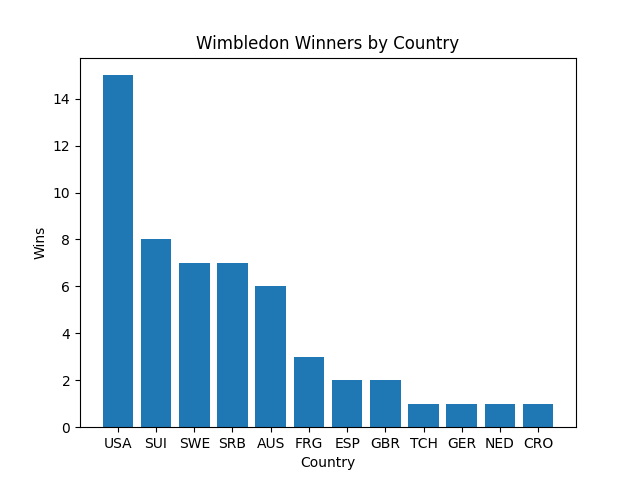
\includegraphics[width=\linewidth]{PS6a_Rann.png}
    \caption{Country Bar}
    \label{fig:image1}
  \end{subfigure}
  \begin{subfigure}[b]{0.3\linewidth}
    \centering
    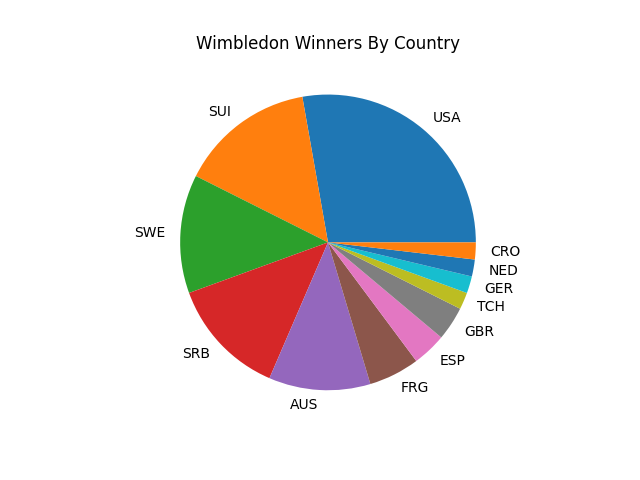
\includegraphics[width=\linewidth]{PS6b_Rann.png}
    \caption{Country Pie}
    \label{fig:image2}
  \end{subfigure}
  \begin{subfigure}[b]{0.3\linewidth}
    \centering
    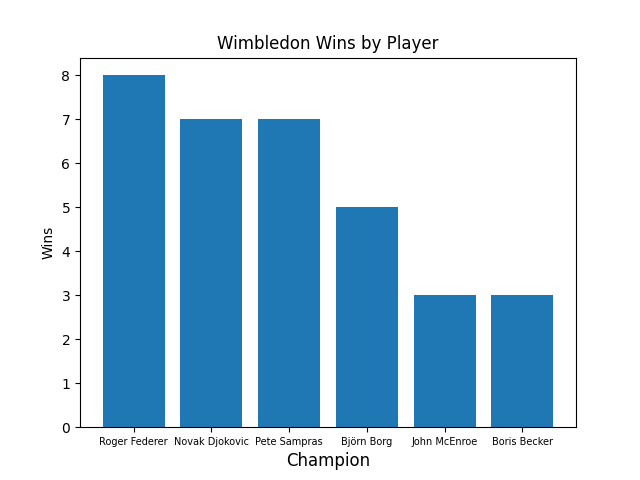
\includegraphics[width=\linewidth]{PS6c_Rann.png}
    \caption{Champion Bar}
    \label{fig:image3}
  \end{subfigure}
  \caption{Wimbledon Champions}
  \label{fig:threeimages}
\end{figure}










\end{document}